% !TEX root = SystemTemplate.tex

\chapter{Overview and concept of operations}

The purpose of this document is to outline the project. That is, it's purpose, the niche it is meant to fill, and it's future.


\section{Scope}
This document covers the details of the project. It describes how it works, what tools it uses, and what has been done so far.


\section{Purpose}
The purpose is to make grading easier for professors and teaching assistants (in particular at the introductory programming level).


\subsection{Major System Component \#1}
Recursive File Searcher

\subsection{Major System Component \#2}
Iterative Executable Tester

\section{Systems Goals}
The primary goal of the project is to aid in the grading of programs. Without a tool to do this, it can be very time-consuming to grade programs that are all meant to be "the same." This is the problem that Assignment Grader is mean to solve.

\section{System Overview and Diagram}
These are the main system components. For clarity, the student's code file has been included in this diagram even though it is an outside resource. See Figure~\ref{systemdiagram} below.

\begin{figure}[tbh]
\begin{center}
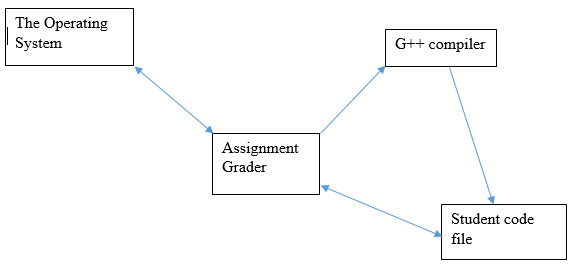
\includegraphics[width=0.75\textwidth]{./diagram}
\end{center}
\caption{System Diagram \label{systemdiagram}}
\end{figure}

\section{Technologies Overview}
Linux (Fedora 19, Ubuntu 13.1) Operating System: Used for basic runtime needs. G+ compiler: used to compile and run both our code and student code. For further information on these two system features, consult Linux documentation.

